% -*- LaTeX -*-
% -*- coding: utf-8 -*-
%
% ~~~~~~~~~~~~~~~~~~~~~~~~~~~~~~~~~~~~~~~~~~~~~~~~~~~~~~~~~~~~~~~~~~~~~~~~~~~~~~
%
%                             michael a.g. aïvázis
%                      california institute of technology
%                      (c) 1998-2010  all rights reserved
%
% ~~~~~~~~~~~~~~~~~~~~~~~~~~~~~~~~~~~~~~~~~~~~~~~~~~~~~~~~~~~~~~~~~~~~~~~~~~~~~~
%

\lecture{Programming with MPI}{20100125}

% --------------------------------------
% template
\begin{frame}[fragile]
%
  \frametitle{Distributed memory parallelism}
%
  \begin{itemize}
%
  \item recall the generic layout of a distributed memory machine
%
    \begin{figure}
      \centering
      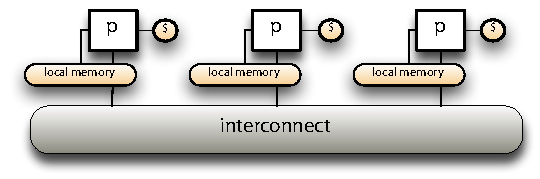
\includegraphics[scale=0.5]{figures/distributed-memory.pdf}
    \end{figure}
    \vspace{-1.0em}
%
    \begin{itemize}
      \item each processor has its own private memory space
      \item processors communicate via the interconnect substrate
    \end{itemize}
%
  \item the programming model
    \begin{itemize}
    \item program consists of a collection of $p$ named processes
      \item each process has its own instruction stream and address space
    \item logically shared data must be partitioned among the processors
    \item communication and synchronization must be orchestrated explicitly 
    \item processes communicate via explicit data exchanges
    \item co\"ordination is implicit in every communication
    \end{itemize}
%
  \end{itemize}
%
\end{frame}

% --------------------------------------
% template
\begin{frame}[fragile]
%
  \frametitle{Blank}
%
  \begin{itemize}
%
  \item 
%
  \end{itemize}
%
\end{frame}

% --------------------------------------
% hello world
\begin{frame}[fragile]
%
  \frametitle{Hello world}
%
  \label{slide:hello-world-mpi}
%
  \begin{C}
#include <mpi.h>
#include <stdio.h>

int main(int argc, char* argv[]) {
    int status;
    int rank, size;

    /* initialize MPI */
    status = MPI_Init(&argc, &argv);
    if (status != MPI_SUCCESS) {
        printf("error in MPI_Init; aborting...\n");
        return status;
    }

    /* all good */
    MPI_Comm_rank(MPI_COMM_WORLD, &rank);
    MPI_Comm_size(MPI_COMM_WORLD, &size);
    printf("hello from %03d/%03d\n", rank, size);

    /* shut down MPI */
    MPI_Finalize();

    return 0;
}
  \end{C}
%
\end{frame}

% end of file 
